\documentclass[11pt]{beamer}
\usepackage{graphicx}
\graphicspath{ {./Images/} }
\setbeamertemplate{caption}[numbered]
\usepackage{caption}
\usepackage{float}
\usepackage{hyperref}
\usepackage{multirow}
\setbeamersize{text margin left=0.5cm,text margin right=0.5cm}
\usepackage{multicol}
\usepackage{listings}
\usepackage{color}
\usepackage{fancyvrb}
\usepackage{booktabs}
\definecolor{dkgreen}{rgb}{0,0.6,0}
\definecolor{gray}{rgb}{0.5,0.5,0.5}
\definecolor{mauve}{rgb}{0.58,0,0.82}
\lstset{
  language=Java,
  aboveskip=3mm,
  belowskip=3mm,
  showstringspaces=false,
  columns=flexible,
  basicstyle={\small\ttfamily},
  numbers=none,
  frame=single,
  numberstyle=\tiny\color{gray},
  keywordstyle=\color{blue},
  commentstyle=\color{dkgreen},
  stringstyle=\color{mauve},
  breaklines=true,
  breakatwhitespace=true,
  tabsize=3,
  fancyvrb=true,
}

\makeatletter
\let\save@measuring@true\measuring@true
\def\measuring@true{%
  \save@measuring@true
  \def\beamer@sortzero##1{\beamer@ifnextcharospec{\beamer@sortzeroread{##1}}{}}%
  \def\beamer@sortzeroread##1<##2>{}%
  \def\beamer@finalnospec{}%
}
\makeatother

\mode<presentation> {
    \usetheme{Warsaw}
    \setbeamertemplate{footline}[page number]
    }
    
\definecolor{violet}{rgb}{0.54, 0.17, 0.89}
\newcommand{\red}[1]{\textcolor{red}{#1}}
\newcommand{\violet}[1]{\textcolor{violet}{#1}}
\newcommand{\green}[1]{\textcolor{green}{#1}}
\newcommand{\sol}{\textbf{Solution}: \pause \newline}

\title[Chapter 08 Notes]{Math 130: Introduction to Programming \\ Chapter 08: A Second Look at Classes and Objects \\ Lecture Notes}
\author{Jesús R. Pérez Cuarenta \\
\href{mailto:jperezcuarenta@swccd.edu}{jperezcuarenta@swccd.edu}
}
\date{}

\begin{document}
\begin{frame}
  \maketitle
\end{frame}

\begin{frame}
\frametitle{Overview}
    \tableofcontents
\end{frame}

\section{Static Class Members, Objects and Methods}
\subsection{Static Class Members}
\begin{frame}[fragile]{Static Members}
    A \red{static} class member \red{belongs to the class}, not objects instantiated from the class.
    \\ \vspace{1em}
    When a value is stored in a static field, it is not stored in an instance of the class. 
    \\ \vspace{1em}
    Static methods do not operate on the fields that belong to any instance of the class. Instead, they can operate only on static fields.
    \\ \vspace{1em} 
    You can think of static fields and static methods as belonging to the class instead of an instance of the class. 
\end{frame}

\begin{frame}[fragile]{Static Fields}
    When a field is declared with the key word static, there will be only one copy of the field in memory, regardless of the number of instances of the class that might exist.
   \\ \vspace{1em}
    A single copy of a class’s static field is shared by all instances of the class.
\end{frame}

\begin{frame}[fragile]{Static Fields}
    \begin{lstlisting}[basicstyle=\ttfamily\footnotesize]
public class StaticDemo {
	public static void main(String[] args) {
		int objectCount;
		Countable object1 = new Countable();
		Countable object2 = new Countable();
		Countable object3 = new Countable();
		objectCount = object1.getInstanceCount();
		System.out.println(objectCount + " instances created."); 
    }}
class Countable {
	private static int instanceCount = 0;
	public Countable() {
		instanceCount++;
		}
	public int getInstanceCount() {
		return instanceCount;
	}}
    \end{lstlisting}
\end{frame}

\begin{frame}[fragile]{Static Methods}
    When a class contains a static method, it isn't necessary for an instance of the class to be created in order to execute the method.
    \begin{lstlisting}
public class MetricDemo {
	public static void main(String[] args) {
		double miles, km;
		miles = 120.0;
		km = Metric.milesToKilometers(miles);
		System.out.println(miles + " miles in km: " + km + " km");
		}
	}
class Metric {
	public static double milesToKilometers(double m) {
		return m * 1.609;
		}
	}
    \end{lstlisting}
\end{frame}

\begin{frame}[fragile]{Static Methods}
    The only limitation that static methods have is that they cannot refer to non-static members of the class.
    \begin{lstlisting}
class SomeClassWithStaticMethod {
    public double x = 1; // NOT a static field
    public static void staticMethodExample() {
        // this is a static method
        System.out.println(x); // this is an error
        }
    }
    \end{lstlisting}
\end{frame}

\subsection{Passing Objects as Arguments to Methods}
\begin{frame}[fragile]{Passing Objects as Arguments to Methods}
    To pass an object as a method argument, you pass an object reference.
    \begin{lstlisting}
public class PassObjectReferenceDemo {
	public static void main(String[] args) {
		boringClass instanceObject = new boringClass();
		printField(instanceObject);
		}
	public static void printField(boringClass inputObject) {
		inputObject.boringMethod();
		}
	}
class boringClass {
	private double boringField = 1;
	public void boringMethod() {
		System.out.println(boringField);
		}
	}
    \end{lstlisting}
\end{frame}

\subsection{Returning Objects from Methods}
\begin{frame}{Passing Objects as Arguments to Methods}
    When a variable is passed as an argument to a method, it is said to be \red{passed by value}. \\ \vspace{1em}
    
    This means that \red{a copy of the variable’s value is passed} into the method’s parameter. \\ \vspace{1em}
    
    When a \violet{reference variable is passed} as an argument to a method the method has access to the object that the variable references. \\ \vspace{1em}
    
    When a method receives an object reference as an argument, it is \violet{possible for the method to modify the contents of the object referenced by the variable}.
\end{frame}

\begin{frame}[fragile]{Returning Objects from Methods}
    \begin{lstlisting}
public class ReturnObjectDemo {
	public static void main(String[] args) {
		// declare reference variable
		GenericObject obj;
		// generate object and assign the reference
		obj = getObject();
		}
	public static GenericObject getObject() {
		return new GenericObject();
		}
	}
class GenericObject {
	// Some fields and methods go here...
	}

    \end{lstlisting}
\end{frame}

\section{Describing, Comparing, and Copying Objects}
\subsection{The \texttt{toString} Method}
\begin{frame}[fragile]{The \texttt{toString} Method}
    Most classes can benefit from having a method named \red{\texttt{toString}}. \\ \vspace{1em}
    Typically, the method \red{returns a string that represents the state of an object}.
    \begin{lstlisting}[basicstyle=\ttfamily\footnotesize]
class Student{
	int num;
	String name;
	String city;
	public Student(int r, String n, String c) {
		num = r;  
		name = n;
		city = c;
	 	}
	 public String toString() {
		 return num + " " + name + " " + city;  
	 	}
	 }        
    \end{lstlisting}
\end{frame}

\begin{frame}[fragile]{The \texttt{toString} Method}
\begin{lstlisting}
public class ToStringDemo {
    public static void main(String[] args) {
        Student x = new Student(1, "John", "Chicago");
        Student y = new Student(2, "Robert", "New York");
        System.out.println(x);
        System.out.println(y);
        System.out.println(x.toString());
        System.out.println(y.toString());
        }
    }
\end{lstlisting}    
\end{frame}

\subsection{Writing an \texttt{equals} Method}
\begin{frame}[fragile]{Writing an \texttt{equals} Method}
    You cannot determine whether two objects contain the same data by comparing them with the \texttt{==} operator.  \\ \vspace{1em}
    The class must have a method such as equals for comparing the contents of objects.
    \begin{lstlisting}[basicstyle=\ttfamily\footnotesize]
 public boolean equals(Student obj) {
     boolean isEqual = false;
     boolean numCheck, nameCheck, cityCheck;
     numCheck = num == obj.num;
     nameCheck = name.equals(obj.name);
     cityCheck = city.equals(obj.city);
     if (numCheck && nameCheck && cityCheck) {
        isEqual = true; 
        }
     return isEqual;
     }
    \end{lstlisting}
\end{frame}

\begin{frame}[fragile]{Writing an \texttt{equals} Method}
\begin{lstlisting}
public class equalsDemo {
	public static void main(String[] args) {
		Student s1 = new Student(1, "John", "Chicago");
		Student s2 = new Student(1, "John", "Chicago");
		System.out.println(s1.equals(s2)); // prints true.
		}
	}
\end{lstlisting}
\end{frame}

\subsection{Methods That Copy Objects}
\begin{frame}[fragile]{Methods that Copy Objects}
    You can simplify the process of duplicating objects by equipping a class with a method that returns a copy of an object. \\ \vspace{1em}
    \textbf{The following does NOT copy the object.}
    \begin{lstlisting}
// Example of a reference copy.
Student x = new Student(1, "Albert", "San Diego");
Student xNew = x; 
    \end{lstlisting}
    The right way to copy objects leverages the existing class constructor.
    \begin{lstlisting}
public Student copy() {
    Student objCopy = new Student(num, name, city);
    return objCopy;
    \end{lstlisting}
Note: There are other ways to copy objects, see your book for more details.
\end{frame}

\section{Aggregation, the \texttt{this} Reference Variable}
\subsection{Aggregation}
\begin{frame}[fragile]{Aggregation}
    \red{Aggregation} occurs when an \red{instance} of a class \red{is a field} in another class. \\ \vspace{1em}
\end{frame}
\begin{frame}[fragile]{Aggregation}
\begin{lstlisting}[basicstyle=\ttfamily\footnotesize]
class Operation {
    double square(double n) {
        return n * n;
        }
    }
class Circle {
    Operation oper;
    double piApprox = 3.1415;
    public static void main(String[] args) {
        Circle circObj = new Circle();
        double out = circObj.area(1.0);
        }
    double area (double radius) {
        oper = new Operation();
        double rSquared = oper.square(radius);
        return piApprox * rSquared;
        }
    }
    \end{lstlisting}
\end{frame}

\subsection{The \texttt{this} Reference Variable}
\begin{frame}[fragile]{The \texttt{this} Reference Variable}
    The \red{\texttt{this}} key word is the name of a reference variable that an object can use to refer to itself. \\ \vspace{1em}
    It is available to all non-static methods.
    We can rewrite a constructor
\begin{lstlisting}
public Stock(String sym, double price) {
    symbol = sym;
    sharePrice = price;
    }
\end{lstlisting}
as
\begin{lstlisting}
public Stock(String symbol, double sharePrice) {
    this.symbol = symbol;
    this.sharePrice = sharePrice;
    }
\end{lstlisting}
\end{frame}

\section{Enumerated Types and Garbage Collection}
\subsection{Enumerated Types}
\begin{frame}[fragile]{Enumerated Types}
    An enumerated data type consists of a set of predefined values. \\ \vspace{1em}
    You can use the data type to create variables that can hold only the values that belong to the enumerated data type. \\ \vspace{1em}
    You use the \texttt{enum} key word to create your own data type and specify the values that belong to that type.
    \begin{lstlisting}
enum Day { SUNDAY, MONDAY, TUESDAY, WEDNESDAY, THURSDAY, FRIDAY, SATURDAY }
    \end{lstlisting}    
\end{frame}

\begin{frame}[fragile]{Enumerated Types}
    An enumerated data type declaration begins with the key word \texttt{enum}, followed by the name of the type, followed by a list of identifiers inside braces. \\ \vspace{1em}

    Previous example:
    \begin{itemize}
        \item Data type: \texttt{Day}
        \item \texttt{enum} constants: \texttt{SUNDAY, MONDAY, TUESDAY, \ldots}
    \end{itemize}
\end{frame}

\begin{frame}[fragile]{Enumerated Types}
    Once you have created an enumerated data type in your program, you can declare variables of that type.
    \begin{lstlisting}
Day workDay = Day.WEDNESDAY;
    \end{lstlisting}
    \noindent 
    \begin{figure}[H]
    \centering
    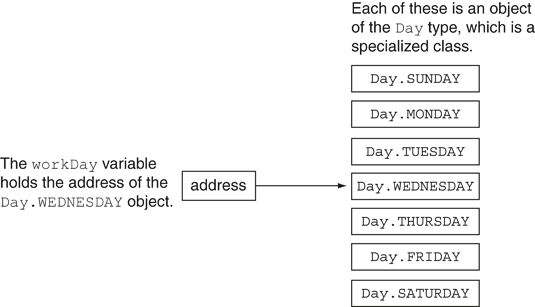
\includegraphics[scale=0.5]{Images/chapter08_section09_EnumVisual.png}
    \end{figure}
\end{frame}

\begin{frame}[fragile]{Enumerated Types}
    Every \texttt{enum} constant comes equipped with a couple of methods. \\ \vspace{1em}
    These methods include: \texttt{toString}, \texttt{ordinal}, \texttt{equals} and \texttt{compareTo}.
    \begin{lstlisting}
enum Day {SUNDAY, MONDAY, TUESDAY, WEDNESDAY, THURSDAY, FRIDAY, SATURDAY};
Day workDay = Day.WEDNESDAY;
Day vacationDay = Day.SUNDAY;
System.out.println(workDay.toString()); // WEDNESDAY
System.out.println(vacationDay.ordinal()); // 0
System.out.println(workDay.equals(Day.WEDNESDAY)); // true
System.out.println(workDay.compareTo(Day.SATURDAY)); // -3
    \end{lstlisting}
\end{frame}

\subsection{Garbage Collection}
\begin{frame}[fragile]{Garbage Collection}
    The Java Virtual Machine runs a process known as the \red{garbage collector}, which removes unreferenced objects from memory. \\ \vspace{1em}
    Motivation:
\begin{lstlisting}
BankAccount account1, account2;
account1 = new BankAccount(500.0);
account2 = account1;
account1 = null;
account2 = null;
// BankAccount object is no longer accessible so remove from memory
// with the garbage collector process.
\end{lstlisting}
\end{frame}

\begin{frame}{The \texttt{finalize} Method}
    If a class has a method named \texttt{finalize}, it is automatically called just before an instance of the class is destroyed by the garbage collector. \\ \vspace{1em}
    The method accepts no arguments and has a \texttt{void} return type. \\ \vspace{1em}
    Note: You cannot predict exactly when the garbage collector will execute. It runs periodically.
\end{frame}

\end{document}

